\chapter{Approfondimenti teorici}\label{chap:approfondimenti_teorici}

\section{Problema della separabilità non lineare nel percettrone}\label{sec:separabilita_non_lineare}
\textit{Questa parte è tratta dal capitolo \ref{chap:primi_modelli}, dove si parla del percettrone nella sezione \ref{sec:modelli_lineari}.}

\paragraph{Definizione (separabilità lineare).}
Sia $X=\{x^{(1)},\ldots,x^{(m)}\}\subset\mathbb{R}^{d}$ e sia $y\in\{0,1\}^{m}$ un insieme di etichette.
Diciamo che i due insiemi di punti $A=\{x^{(i)}:y^{(i)}=1\}$ e $B=\{x^{(i)}:y^{(i)}=0\}$ sono \emph{linearmente separabili} se esistono $w\in\mathbb{R}^{d}$ e $b\in\mathbb{R}$ tali che
\[
w^\top x \;>\; b \quad \forall x\in A,
\qquad
w^\top x \;<\; b \quad \forall x\in B.
\]
Equivalente: esiste un iperpiano $w^\top x=b$ la cui parte positiva contiene tutti i punti di $A$ e la parte negativa tutti i punti di $B$.

\paragraph{Quante funzioni booleane sono linearmente separabili?}
Per $m$ argomenti binari esistono $2^{2^{m}}$ funzioni booleane possibili; solo una parte è realizzabile con un singolo classificatore lineare.
Dati noti:
\[
\begin{array}{lcl}
m=2 &\Rightarrow& 14 \text{ su } 16 \text{ sono separabili linearmente},\\[2pt]
m=3 &\Rightarrow& 104 \text{ su } 256 \text{ sono separabili linearmente},\\[2pt]
m=4 &\Rightarrow& 1882 \text{ su } 65536 \text{ sono separabili linearmente}.
\end{array}
\]
Non esiste una formula chiusa semplice che dia, in funzione di $m$, quante funzioni sono linearmente separabili; tuttavia si osserva che, all’aumentare di $m$, la \emph{frazione} di funzioni separabili decresce rapidamente.

\paragraph{Dicotomie di un insieme di punti.}
Dato $X=\{x^{(1)},\ldots,x^{(m)}\}\subset\mathbb{R}^{d}$, le possibili etichettature (o \emph{dicotomie}) sono $2^{m}$:
\[
\mathcal{Y}=\{0,1\}^{m} .
\]
Solo una parte di queste dicotomie è realizzabile mediante una frontiera lineare. Con $d$ fissata, il numero di dicotomie realizzabili cresce in modo polinomiale in $m$ (ordine al piu $m^{d}$), mentre il totale cresce esponenzialmente ($2^{m}$); di conseguenza,
\[
\Pr\{\text{dicotomia separabile linearmente}\}\;\longrightarrow\;0
\quad\text{quando } m \gg d .
\]

\begin{figure}[htbp]
	\centering
	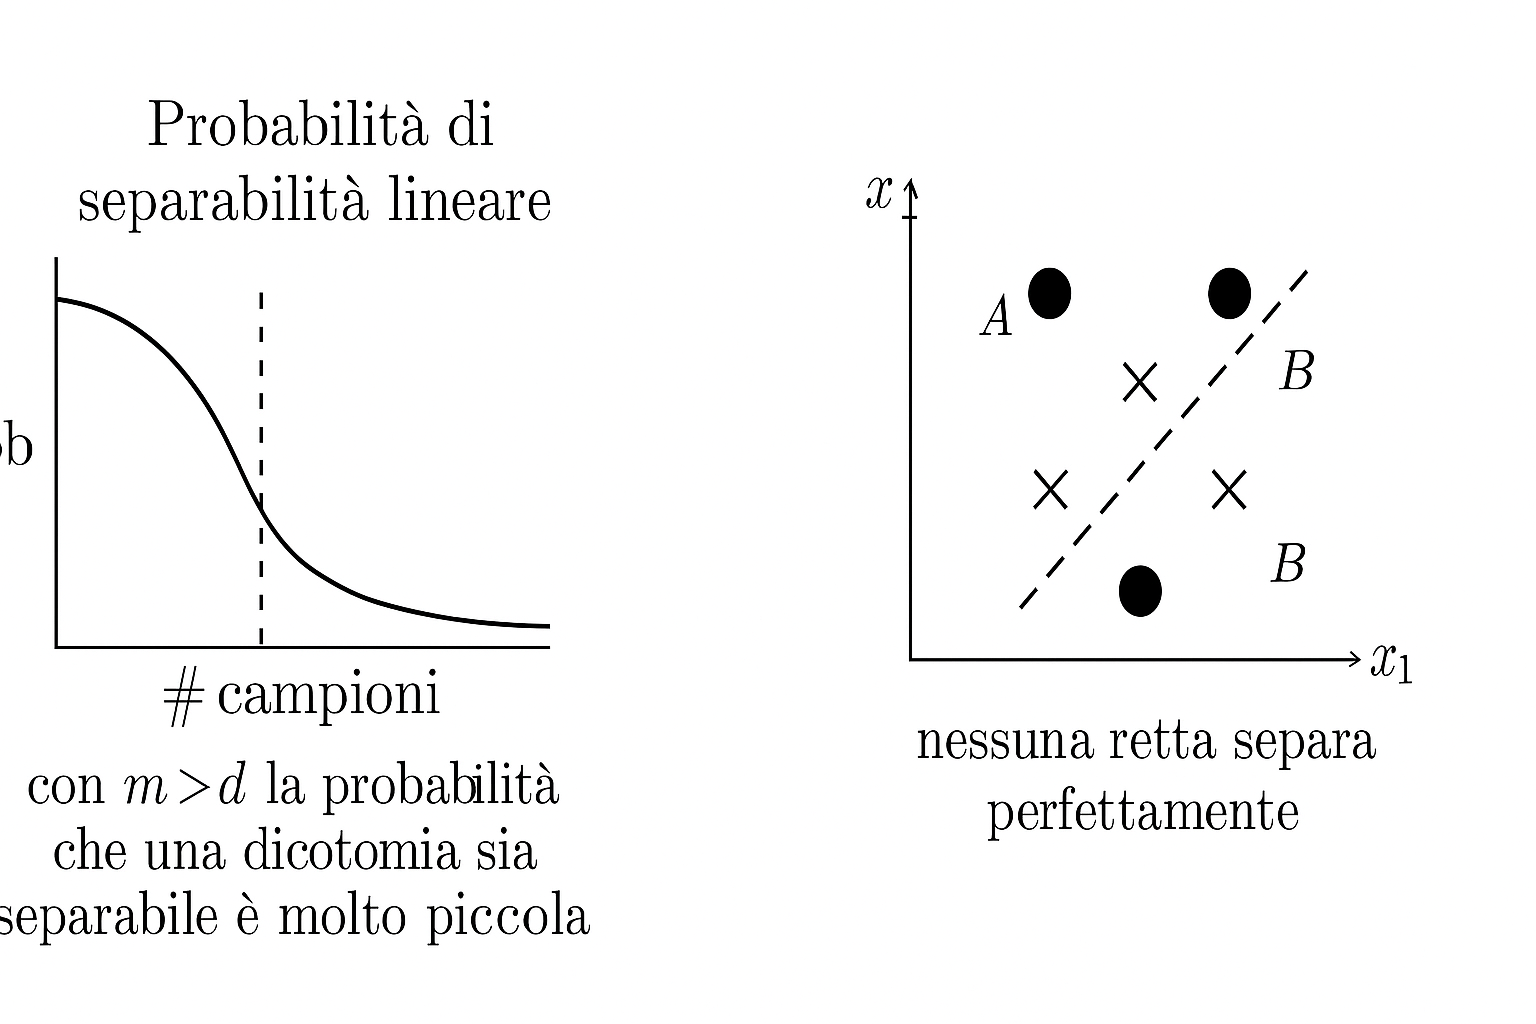
\includegraphics[width=0.7\linewidth]{images/non_linear_separation-probability.png}
	\caption{Separabilità non lineare. A sinistra: andamento qualitativo della probabilità che una dicotomia sia linearmente separabile al crescere del numero di campioni \(m\) (con dimensione \(d\) fissata); a destra: esempio in \(\mathbb{R}^2\) di punti non separabili con un singolo iperpiano.}
	\label{fig:nonlinear-separability}
\end{figure}

Intuitivamente: se il numero di campioni cresce molto a parità di dimensione $d$, è sempre meno probabile che una separazione perfetta con una sola retta/iperpiano esista.


\section{Generalizzazione funzione di costo del softmax}\label{sec:softmax_generalizzazione_logistica}
\textit{Questa parte è tratta dal capitolo \ref{chap:classificazione} nella sezione \ref{sec:proprieta_softmax}.}

\bigskip
\noindent
Il modello softmax è una generalizzazione della regressione logistica multiclasse, si può infatti dimostrare che la funzione di costo del softmax riduce a quella della regressione logistica binaria per $K=2$ classi.
Ricordiamo che la funzione di costo del softmax è:
\[
J(\vartheta)
= -\frac{1}{m}\sum_{i=1}^{m}\sum_{c=0}^{K-1}
\mathbf{1}\{y^{(i)}=c\}\,\log\!\big(h_{\vartheta}^{(c)}(x^{(i)})\big)
+\frac{\lambda}{2}\sum_{c=0}^{K-1}\sum_{j=1}^{n}(\vartheta_j^{(c)})^2,
\]

É facile vedere che, per $K=2$ (senza regolarizzazione) vale:
\begin{align*}
J(\vartheta)
&= -\frac{1}{m}\sum_{i=1}^{m}\sum_{c=0}^{1}
\mathbf{1}\{y^{(i)}=c\}\,\log\!\big(h_{\vartheta}^{(c)}(x^{(i)})\big)\\
&= -\frac{1}{m}\sum_{i=1}^{m}
\Big[\mathbf{1}\{y^{(i)}=0\}\log h_{\vartheta}^{(0)}(x^{(i)})
     +\mathbf{1}\{y^{(i)}=1\}\log h_{\vartheta}^{(1)}(x^{(i)})\Big]\\
&= -\frac{1}{m}\sum_{i=1}^{m}
\Big[(1-y^{(i)})\log h_{\vartheta}^{(0)}(x^{(i)})
     +y^{(i)}\log h_{\vartheta}^{(1)}(x^{(i)})\Big]\\
&= -\frac{1}{m}\sum_{i=1}^{m}
\Big[(1-y^{(i)})\log\!\big(1-h_{\vartheta}^{(1)}(x^{(i)})\big)
     +y^{(i)}\log h_{\vartheta}^{(1)}(x^{(i)})\Big],
\end{align*}

dove si è usata la normalizzazione della softmax $h_{\vartheta}^{(0)}(x)+h_{\vartheta}^{(1)}(x)=1$.
Questa è esattamente la loss della regressione logistica binaria: dunque la regressione logistica è un caso particolare della softmax.

Si può ulteriormente dimostrare che il softmax è una generalizzazione della regressione logistica multiclasse usando una sua proprietà principale: l'\emph{overparametrizzazione}. Per $K=2$:
\[
h_{\vartheta}(x)=
\begin{bmatrix}
\dfrac{e^{\vartheta^{(0)\!\top}x}}{e^{\vartheta^{(0)\!\top}x}+e^{\vartheta^{(1)\!\top}x}}\\[6pt]
\dfrac{e^{\vartheta^{(1)\!\top}x}}{e^{\vartheta^{(0)\!\top}x}+e^{\vartheta^{(1)\!\top}x}}
\end{bmatrix}
=
\begin{bmatrix}
\dfrac{e^{(\vartheta^{(0)}-\vartheta^{(1)})^\top x}}{e^{(\vartheta^{(0)}-\vartheta^{(1)})^\top x}+e^{\mathbf 0^\top x}}\\[6pt]
\dfrac{e^{(\vartheta^{(1)}-\vartheta^{(1)})^\top x}}{e^{(\vartheta^{(0)}-\vartheta^{(1)})^\top x}+e^{\mathbf 0^\top x}}
\end{bmatrix}
=
\begin{bmatrix}
\dfrac{e^{\Delta^\top x}}{1+e^{\Delta^\top x}}\\[6pt]
\dfrac{1}{1+e^{\Delta^\top x}}
\end{bmatrix},
\qquad \Delta=\vartheta^{(0)}-\vartheta^{(1)}.
\]
Ponendo \(\mathbf w=\vartheta^{(1)}-\vartheta^{(0)}=-\Delta\) e
\(\sigma(z)=\dfrac{1}{1+e^{-z}}\) si ottiene
\[
h_{\vartheta}(x)=
\begin{bmatrix}
1-\sigma(\mathbf w^\top x)\\[4pt]
\sigma(\mathbf w^\top x)
\end{bmatrix}.
\]

\noindent
Quindi, per $K=2$, il softmax riduce alla regressione logistica binaria.

\section{Dimostrazione del teorema del margine a 1}\label{sec:teorema_margine_1}
\textit{Questa parte è tratta dal capitolo \ref{chap:svm} nella sezione \ref{sec:svm_traditional_derivation}.}

\bigskip
\noindent
Imponiamo $\|w\| = 1$. Questo può essere scritto come $ \displaystyle w = \frac{w'}{\|w'\|}$, dove $w'$ è un vettore di parametri qualsiasi non normalizzato. Sostituendo nella formulazione iniziale, otteniamo

$$
y \left(\Big\langle \frac{w'}{\|w'\|}, x\Big\rangle + b\right) \geq r
$$

Noto che $r \geq 0$ in quanto una distanza euclidea, possiamo andare a dividere l'intero vincolo per $r$. Otteniamo:

$$
y \left(\Big\langle \frac{w'}{\|w'\|r}, x\Big\rangle + \underbrace{\frac{b}{r}}_{b''} \right) \geq 1
$$

Bene, adesso definiamo $\displaystyle \|w''\|
= \left\|\frac{w'}{\|w'\| r}\right\|
= \frac{1}{r}\,\frac{\|w'\|}{\|w'\|}
= \frac{1}{r}, \Rightarrow r = \frac{1}{\| w''\|}$. \\
Per facilitare la dimostrazione, imponiamo di dover massimizzare $r^2$, ossia  $\displaystyle\frac{1}{\|w''\|^2}$. Tuttavia, massimizzare questo valore, significa minimizzare  $\|w''\|^2$, o, per semplificare il lavorare con le derivate, equivale a minimizzare $\displaystyle\frac{1}{2} \|w''\|^2$.


$$
\min_{w'',b''} \frac12\|w\|^2 \qquad y (\langle w'', x\rangle + b'') \geq 1
$$
Data questa totale equivalenza, abbiamo dimostriamo il teorema.


\section{Dual SVM}\label{sec:dual_svm_approfondimento}

\textit{Questa parte è tratta dal capitolo \ref{chap:svm} nella sezione \ref{sec:dual_svm}.}

\bigskip
\noindent
La formulazione di SVM descritta in precedenza, è nota come primal SVM. Ha variabili $w$ e $b$, e $w$ è di dimensione pari a $x \in \mathbb{R}^D$, con $D$ features. Ne consegue che il problema di ottimizzazione cresce linearmente all'aumentare del numero di features. La seguente formulazione, crescerà invece col numero di esempi del dataset, non dipendendo più dal numero di features. Sarà inoltre semplice applicarne dei kernel, per separare meglio dati non linearmente separabili. Chiarememo questa formulazione \textbf{Dual SVM}, e si presenterà così:

$$
\begin{aligned}
	&\min_{\alpha} && 
	\frac{1}{2} \sum_{i=1}^{N} \sum_{j=1}^{N} 
	y_i y_j \alpha_i \alpha_j \langle x_i, x_j \rangle
	- \sum_{i=1}^{N} \alpha_i \\
	&\text{soggetto a} && 
	\sum_{i=1}^{N} y_i \alpha_i = 0, \\
	& && 0 \le \alpha_i \le C \quad \text{per } i = 1,\dots, N .
\end{aligned}
$$

\paragraph{Prerequisito matematico: Lagrangiani}
Data una funzione $f$ da ottimizzare, e un insieme di condizioni $g_1, \dots, g_n$, un \textbf{Lagrangiano} è una funzione $\mathcal{L}(f,g_1, \dots, g_n, \alpha_1, \dots, \alpha_n)$ che incorpora le condizioni del problema di ottimizzazione:

$$
\mathcal{L}(f,\alpha_1,\ldots,\alpha_n)
= f(x_1,\ldots,x_k) - \sum_{i=1}^{n} \alpha_i\, g_i(x_1,\ldots,x_k)
$$

Ad esempio, se $f(w) = \displaystyle\frac{w^2}{2}$ e $\displaystyle g_1(w,x) : wx-1 \geq 0$, allora

$$
\mathcal{L}(w,\alpha) = \frac{w^2}{2} - \alpha(wx-1), \quad \alpha \geq 0
$$

Si calcolano le derivate parziali del Lagrangiano rispetto alle variabili
del problema, in questo esempio $w$ e $\alpha$, e si impongono nulle.
Si ottiene così un sistema di equazioni le cui soluzioni soddisfano
le condizioni di ottimalità (condizioni di stazionarietà).

Il Lagrangiano del problema è

$$
\mathcal{L}(w,\alpha)
=
\frac{1}{2} w^{2}
-
\alpha (wx - 1),
\qquad
\alpha \ge 0.
$$

Calcoliamo le derivate parziali.

Derivando rispetto a $w$:

$$
\frac{\partial \mathcal{L}}{\partial w}
=
w - \alpha x.
$$

Imponendo la condizione di stazionarietà otteniamo

$$
w - \alpha x = 0
\quad \Rightarrow \quad
w = \alpha x.
$$

Derivando rispetto a $\alpha$:

$$
\frac{\partial \mathcal{L}}{\partial \alpha}
=
-(wx - 1).
$$

Imponendo la derivata nulla:

$$
wx - 1 = 0.
$$

\subsection{Convex duality con Moltiplicatori di Lagrange}

Riprendiamo le variabili della formulazione primale: $w, b, \xi$.
Introduciamo i moltiplicatori di Lagrange $\alpha_n \ge 0$
associati ai vincoli

\[
y_n(\langle w,x_n\rangle + b) \ge 1 - \xi_n,
\]

e i moltiplicatori $\gamma_n \ge 0$ associati ai vincoli
$\xi_n \ge 0$.

Il Lagrangiano è

\[
\begin{aligned}
\mathcal{L}(w,b,\xi,\alpha,\gamma)
&=
\frac{1}{2}\|w\|^2
+ C \sum_{n=1}^{N} \xi_n
\\
&\quad
- \sum_{n=1}^{N}
\alpha_n
\big(
y_n(\langle w,x_n\rangle + b) - 1 + \xi_n
\big)
- \sum_{n=1}^{N} \gamma_n \xi_n .
\end{aligned}
\]

Deriviamo rispetto alle variabili primali.

\[
\frac{\partial \mathcal{L}}{\partial w}
=
w - \sum_{n=1}^{N} \alpha_n y_n x_n,
\]

\[
\frac{\partial \mathcal{L}}{\partial b}
=
- \sum_{n=1}^{N} \alpha_n y_n,
\]

\[
\frac{\partial \mathcal{L}}{\partial \xi_n}
=
C - \alpha_n - \gamma_n.
\]

Imponendo le condizioni di stazionarietà otteniamo

\[
w = \sum_{n=1}^{N} \alpha_n y_n x_n,
\]

\[
\sum_{n=1}^{N} \alpha_n y_n = 0,
\]

\[
C - \alpha_n - \gamma_n = 0.
\]

Dalla terza equazione segue che

\[
0 \le \alpha_n \le C.
\]

Sostituendo l'espressione di $w$ nel Lagrangiano
ed eliminando $\xi_n$ e $\gamma_n$ tramite le condizioni
di stazionarietà, otteniamo il problema duale.

Il duale consiste nel massimizzare rispetto agli $\alpha_n$:

\[
\begin{aligned}
\max_{\alpha} \quad
& \sum_{n=1}^{N} \alpha_n
-
\frac{1}{2}
\sum_{i=1}^{N}\sum_{j=1}^{N}
\alpha_i \alpha_j y_i y_j
\langle x_i,x_j\rangle
\\
\text{soggetto a} \quad
& \sum_{n=1}^{N} \alpha_n y_n = 0, \\
& 0 \le \alpha_n \le C.
\end{aligned}
\]

\paragraph{Box Constraints} Indichiamo con questo nome l'insieme di disuguaglianze $0 \le \alpha_i \le C \quad\text{per } i=1,\dots,N$. Questi, limitano il vettore dei moltiplicatori di Lagrange $\alpha = [\alpha_1, \dots, \alpha_N]^\top\in \mathbb{R}^N$ in una "scatola" definita tra 0 e $C$ per ogni asse.

\paragraph{Dal Duale al Primale} Una volta trovati i parametri $\alpha$, possiamo ottenere i parametri $w$ usando il \textbf{representer theorem}.

$$
w = \sum_{n=1}^{N} \alpha_n y_n x_n
$$

e indicheremo il suo valore ottimale con $w^*$. 
Per determinare $b^*$, utilizziamo la condizione di margine
valida per i support vector tali che $0 < \alpha_n < C$.
Per questi punti vale infatti

\[
y_n(\langle w^*, x_n\rangle + b^*) = 1.
\]

Da cui possiamo ricavare

\[
b^* = y_n - \langle w^*, x_n\rangle.
\]

\section{L'idea dietro le Random Ferns}\label{sec:random_ferns_idea}
\textit{Questa parte è tratta dal capitolo \ref{chap:random_forest} nella sezione \ref{sec:random_ferns}.}

\bigskip
\noindent
L’idea di fondo è riformulare il problema del matching tra keypoint come un problema di classificazione probabilistica. 
Ogni keypoint stabile osservato in fase di training viene considerato come una classe $c_i$. 
Data una nuova patch $x$, vogliamo assegnarla alla classe più probabile:

\[
\hat{c} = \arg\max_{c_i} P(C = c_i \mid f_1, \dots, f_N)
\]

dove $f_1, \dots, f_N$ sono feature binarie calcolate sulla patch.

\subsection{Feature binarie}

Le feature utilizzate sono estremamente semplici: ciascuna consiste in un confronto tra l’intensità di due pixel della patch:

\[
f_j =
\begin{cases}
1 & \text{se } I(d_{j,1}) < I(d_{j,2}) \\
0 & \text{altrimenti}
\end{cases}
\]

Queste feature sono scelte casualmente e in numero elevato ($N$ può essere dell’ordine di alcune centinaia). 
La discriminatività non deriva dalla singola feature, ma dall’aggregazione di molte di esse.

\subsection{Formulazione probabilistica}

Applicando il teorema di Bayes:

\[
P(C = c_i \mid f_1, \dots, f_N)
=
\frac{
P(f_1, \dots, f_N \mid C = c_i)\, P(C = c_i)
}{
P(f_1, \dots, f_N)
}
\]

Assumendo prior uniformi sulle classi e ignorando il denominatore (comune a tutte), la decisione si riduce a:

\[
\hat{c} = \arg\max_{c_i} P(f_1, \dots, f_N \mid C = c_i)
\]

Il problema è che modellare la distribuzione congiunta completa richiederebbe stimare $2^N$ configurazioni per classe, il che è costoso per $N$ grande.

\subsection{Approccio Semi-Naive Bayes}

Per rendere il problema trattabile si introduce un compromesso tra indipendenza totale e modellazione completa.

Le $N$ feature vengono suddivise in $M$ gruppi (detti \emph{ferns}), ciascuno di dimensione $S$:

\[
F_k = \{ f_{\sigma(k,1)}, \dots, f_{\sigma(k,S)} \}
\]

Si assume indipendenza tra gruppi diversi, ma si modella la distribuzione congiunta completa all’interno di ciascun gruppo:

\[
P(f_1, \dots, f_N \mid C=c_i)
=
\prod_{k=1}^{M}
P(F_k \mid C=c_i)
\]

Ogni fern può assumere $2^S$ configurazioni binarie. 
Il numero di parametri per classe diventa quindi:

\[
M \cdot 2^S
\]

che è gestibile per valori tipici come $S \approx 10$-$11$ e $M$ dell’ordine di alcune decine.

\subsection{Stima delle probabilità}

Durante il training si stimano le probabilità

\[
P(F_k = r \mid C=c_i)
\]

tramite conteggi sulle patch di training (spesso generate applicando trasformazioni affini casuali per aumentare la robustezza).

Per evitare probabilità nulle si utilizza una regolarizzazione di tipo additivo:

\[
P(F_k = r \mid C=c_i)
=
\frac{N_{r,c_i} + \alpha}
     {N_{c_i} + 2^S \alpha}
\]

dove $\alpha > 0$ è un parametro di smoothing.
